% Generated by code/ch12_grape.py -- do not edit by hand.
\definecolor{qocA}{rgb}{0.00,0.45,0.70}
\definecolor{qocB}{rgb}{0.90,0.60,0.00}
\definecolor{qocC}{rgb}{0.00,0.62,0.45}
\definecolor{qocD}{rgb}{0.80,0.40,0.00}
\definecolor{qocE}{rgb}{0.80,0.60,0.70}
\definecolor{qocF}{rgb}{0.35,0.70,0.90}
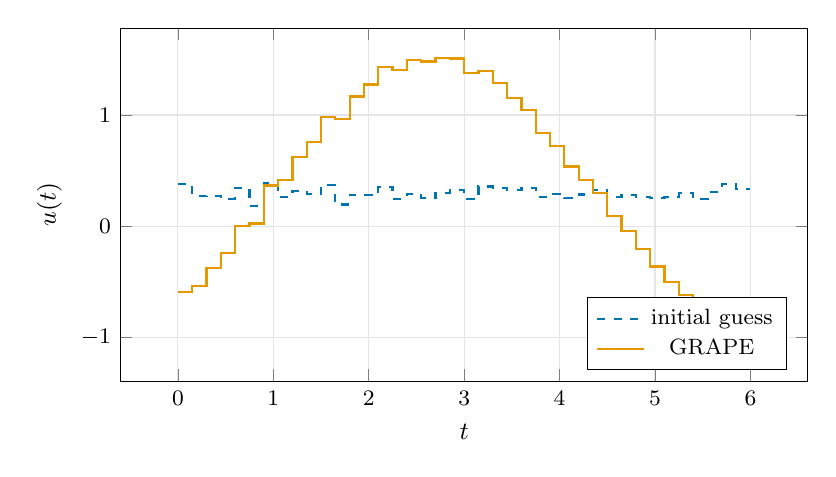
\begin{tikzpicture}[]
\begin{axis}[width=0.85\linewidth, height=0.5\linewidth, xlabel={$t$}, ylabel={$u(t)$}, legend pos=south east, legend style={font=\footnotesize}, tick label style={font=\footnotesize}, label style={font=\small}, grid=major, grid style={gray!20}]
\addplot[thick, qocA, dashed, const plot] coordinates {(0,0.38122) (0.15,0.26941) (0.3,0.27359) (0.45,0.24635) (0.6,0.34327) (0.75,0.18492) (0.9,0.38724) (1.05,0.26194) (1.2,0.31595) (1.35,0.28753) (1.5,0.37311) (1.65,0.19699) (1.8,0.28388) (1.95,0.2808) (2.1,0.35669) (2.25,0.24501) (2.4,0.29138) (2.55,0.25611) (2.7,0.30211) (2.85,0.32914) (3,0.24497) (3.15,0.35724) (3.3,0.34508) (3.45,0.32512) (3.6,0.34504) (3.75,0.26581) (3.9,0.29386) (4.05,0.25321) (4.2,0.28661) (4.35,0.32652) (4.5,0.26542) (4.65,0.28016) (4.8,0.26564) (4.95,0.25774) (5.1,0.26644) (5.25,0.29937) (5.4,0.24413) (5.55,0.31172) (5.7,0.38299) (5.85,0.3371) (6,0.3371)};
\addplot[thick, qocB, const plot] coordinates {(0,-0.58815) (0.15,-0.53555) (0.3,-0.3763) (0.45,-0.24204) (0.6,0.0044582) (0.75,0.025893) (0.9,0.36759) (1.05,0.41795) (1.2,0.62508) (1.35,0.75493) (1.5,0.97909) (1.65,0.96194) (1.8,1.1662) (1.95,1.2751) (2.1,1.4346) (2.25,1.4055) (2.4,1.4924) (2.55,1.4812) (2.7,1.5157) (2.85,1.507) (3,1.3754) (3.15,1.396) (3.3,1.2866) (3.45,1.1543) (3.6,1.0448) (3.75,0.83816) (3.9,0.72032) (4.05,0.5373) (4.2,0.41734) (4.35,0.30179) (4.5,0.096268) (4.65,-0.041713) (4.8,-0.20488) (4.95,-0.36102) (5.1,-0.50086) (5.25,-0.61705) (5.4,-0.80859) (5.55,-0.88745) (5.7,-0.95801) (5.85,-1.126) (6,-1.126)};
\legend{initial guess, GRAPE, 150 iterations}
\end{axis}
\end{tikzpicture}
